\documentclass[10pt]{beamer}

\usetheme{metropolis}
\usepackage{appendixnumberbeamer}

\usepackage{booktabs}
\usepackage[scale=2]{ccicons}

\usepackage{pgfplots}
\usepgfplotslibrary{dateplot}

\usepackage{xspace}
\newcommand{\themename}{\textbf{\textsc{metropolis}}\xspace}
\usepackage{tabularx}

\usepackage[utf8]{inputenc}
\usepackage[brazilian]{babel}

\usepackage{blindtext}

\title{}
\subtitle{Proposta de uma abordagem para a detecção online de mudanças de conceito em fluxos contínuos de dados}
\date{}
\author{\textbf{Discente:} Ruivaldo Neto \newline \textbf{Orientador:} Ricardo Rios}
\institute{Universidade Federal da Bahia \newline Departamento de Ciência da Computação \newline Programa de Pós-Graduação em Ciência da Computação \newline\newline Contato: rneto@rneto.dev \newline\newline 14 de Junho de 2019}

\titlegraphic{%
  \begin{picture}(0,0)
    \put(330, 0){\makebox(0,0)[rt]{
\includegraphics[scale=0.25]{logo.png}}}
  \end{picture}
}

\begin{document}

\maketitle

\begin{frame}{Roteiro}
  \setbeamertemplate{section in toc}[sections numbered]
  \begin{minipage}{\textwidth}
    \tableofcontents
  \end{minipage}
\end{frame}

\section{Introdução}

%\subsection{Contexto e Motivação}

\begin{frame}{Contexto e Motivação}
    \begin{itemize}
        \item<1 -> Avanços tecnológicos recentes favoreceram o aumento no volume de dados produzidos por sistemas computacionais.
        \item<2 -> Muitos desses dados são produzidos na forma de sequências ininterruptas e potencialmente infinitas, denominadas \alert{Fluxos Contínuos de Dados (FCDs)} \cite{Aggarwal:2006:DSM:1196418}.
      \end{itemize}
\end{frame}

\begin{frame}{Contexto e Motivação}
    \begin{itemize}
        \item<1 -> Para extrair informações úteis desses grandes conjuntos, técnicas da área de Aprendizado de Máquina (AM) têm sido aplicadas.
        \item<2 -> Contudo, além das restrições impostas pelos fluxos contínuos, estas técnicas também devem lidar com alterações no contexto do processo gerador do fluxo e/ou na distribuição dos dados. 
        \item<3 -> Estas alterações são denominadas \alert{Mudanças de Conceito} e podem impactar a acurácia do modelo.
      \end{itemize}
\end{frame}

\begin{frame}{Contexto e Motivação}
    \begin{itemize}
        \item<1 -> Inicialmente, a atualização periódica do modelo foi utilizada como técnica para mitigar a perda causada por essas mudanças.
        \item<2 -> Com o avanço da pesquisa, métodos de detecção de mudança baseados em monitoramento foram propostos.
      \end{itemize}
\end{frame}


\begin{frame}{Contexto e Motivação}
    \begin{itemize}
        \item<1 -> Os métodos existentes na literatura apresentam limitações ao serem aplicados em cenários com fluxos contínuos de dados.
        \item<2 -> As principais limitações são: a necessidade de rótulação e/ou tempo de resposta elevado.
        \item<3 -> Visando mitigá-las, este trabalho discute uma abordagem baseada em Redes de Função de Base Radial (RBF) para detecção de mudanças de conceito em FCDs.
      \end{itemize}
\end{frame}

%\subsection{Hipótese}

\begin{frame}{Hipótese}

    \begin{center}
        \textit{``A aplicação de Redes de Função de Base Radial em fluxos contínuos de dados permite a detecção de mudanças de conceito em tempo de execução, de forma computacionalmente eficiente e independente de rótulos.''}
    \end{center}

\end{frame}

\begin{frame}{Hipótese}
    \begin{itemize}
        \item<1 -> O objetivo deste trabalho é a validação da hipótese. Para tanto, um novo método de detecção, baseado em redes RBF, será desenvolvido.
        \item<2 -> O método será validado através de comparações com o estado da arte.
        \item<3 -> Dois conjuntos de dados serão utilizados nos experimentos, um sintético e outro oriundo de uma aplicação do mundo real.
      \end{itemize}
\end{frame}

\section{Revisão Bibliográfica}

%\subsection{Fluxos Contínuos de Dados e Aprendizado de Máquina}

\begin{frame}{Fluxos Contínuos de Dados e Aprendizado de Máquina}
    \begin{itemize}
        \item<1 -> \alert{Fluxos Contínuos de Dados (FCDs)} podem ser definidos como sequências ininterruptas e potencialmente infinitas de eventos \cite{Aggarwal:2006:DSM:1196418}
        \item<2 -> Estes fluxos não podem ser armazenados em sua totalidade e, por serem de alta frequência, devem ser analisados em tempo real.
        \item<3 -> Algoritmos supervisionados \cite{Domingos:2000:MHD:347090.347107, Bifet:2013:EDS:2480362.2480516, Wang:2003:MCD:956750.956778, Aggarwal:2004:DCD:1014052.1014110, Gama:2003:ADT:956750.956813} e não-supervisionados \cite{Aggarwal:2003:FCE:1315451.1315460, Ackermann:2012:SCA:2133803.2184450, Kranen:2011:CIM:2134350.2134352} foram adaptados para atenderem a essas restrições.
        \item<4 -> Entretanto, o contexto do processo gerador ou a distribuição dos dados gerados podem sofrer alterações.
        \item<5 -> Estas alterações são denominadas \alert{mudanças de conceito} e podem impactar as técnicas de aprendizado aplicadas.
      \end{itemize}
\end{frame}

%\subsection{Mudança de Conceito}

\begin{frame}{Mudança de Conceito}
    \begin{itemize}
        \item<1 -> A Teoria Bayesiana de Decisão \cite{Duda:2000:PC:954544} é comumente utilizada para descrever a tarefa de classificação.
        \item<2 -> Baseando-se nesta teoria e considerando que $p_{t_0}$ e $p_{t_1}$ denotam as distribuições de probabilidades conjuntas nos instantes $t_0$ e $t_1$, é possível afirmar que há mudança de conceito entre os instantes $t_0$ e $t_1$ se:
        \begin{equation} \label{eq:3}
            {\exists}X : p_{t_0}(X, c) \ne p_{t_1}(X, c)
        \end{equation}
        \item<3 -> Um conjunto de dados possui resultados esperados legítimos em $t_0$, mas este mesmo conjunto passa a ter resultados esperados diferentes, também legítimos, em $t_1$ \cite{Kolter:2007:DWM:1314498.1390333}.
    \end{itemize}
\end{frame}

\begin{frame}{Mudança de Conceito}
    \begin{itemize}
        \item<1 -> As mudanças de conceito podem ser categorizadas como virtuais ou reais \cite{Gama:2014:SCD:2597757.2523813}.
        \item<2 -> As mudanças virtuais são causadas por alterações na probabilidade a priori das classes, $P(c)$, e não alteram os conceitos-alvo.
        \item<3 -> Enquanto que as mudanças de conceito reais surgem a partir de alterações na probabilidade a posteriori, $p(c|X)$, e modificam os resultados esperados.
    \end{itemize}
\end{frame}

\begin{frame}{Mudança de Conceito}
\begin{figure}[H]
    \begin{center}
        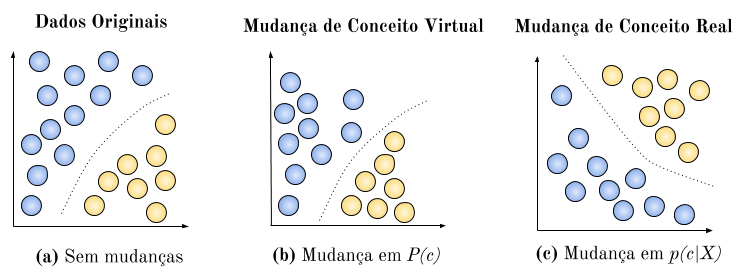
\includegraphics[scale=0.5]{../text/imagens/concept_drift.png}
        \caption{Mudança de Conceito Virtual vs. Mudança de Conceito Real}
        \label{fig:real_and_virtual_concept_drift}
    \end{center}
\end{figure}
\end{frame}

\begin{frame}{Mudança de Conceito}
    \begin{itemize}
        \item<1 -> As mudanças de conceito podem podem ocorrer de forma abrupta, gradual, incremental ou recorrente.
    \end{itemize}
\end{frame}

\begin{frame}{Mudança de Conceito}
\begin{figure}[H]
    \begin{center}
        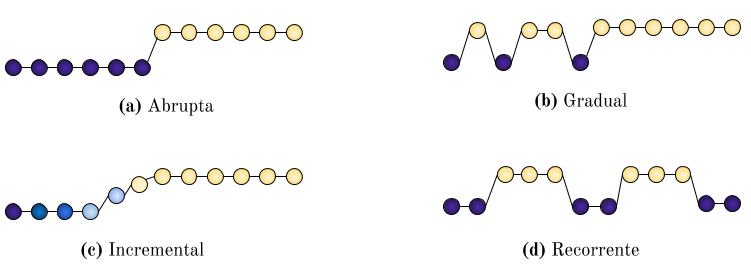
\includegraphics[scale=0.5]{imagens/concept_drift_patterns.png}
        \caption{Padrões de ocorrência de Mudanças de Conceito}
        \label{fig:concept_drift_patterns}
    \end{center}
    \end{figure}
\end{frame}

\begin{frame}{Mudança de Conceito}
    \begin{itemize}
        \item<1 -> O fenômeno mudança de conceito tem sido estudado em diferentes comunidades de pesquisa, incluindo Mineração de Dados, Aprendizado de Máquina, Estatística e Recuperação de Informação \cite{Zliobaite:2010}. Contudo, o tema apresenta diferentes nomeclaturas em cada comunidade.
    \end{itemize}
\end{frame}

\begin{frame}{Mudança de Conceito}
    \begin{table}[!ht]
        \caption{Terminologia - Mudança de Conceito \cite{Zliobaite:2010}}
        \label{tbl:taxonomy}
        \centering
        \resizebox{\textwidth}{!}{%
        \begin{tabular}[t]{ll}
        \toprule
        Área & Termos \\
        \midrule
        Mineração de Dados                  & Mudança de Conceito                        \\
        Aprendizado de Máquina              & Mudança de Conceito, Mudança de Covariável \\
        Computação Evolucionária            & Ambiente Evolutivo, Ambiente em Mudança    \\
        IA e Robótica                       & Ambiente Dinâmico                          \\
        Estatística, Séries Temporais      & Não Estacionário                           \\
        Recuperação de Informação           & Evolução Temporal                          \\
        \bottomrule
        \end{tabular}%
        }
    \end{table}
\end{frame}

%\subsection{Redes de Função de Base Radial}

\begin{frame}{Redes de Função de Base Radial}
    \begin{itemize}
        \item<1 -> A
        \item<2 -> B
        \item<3 -> C
        \item<4 -> D
      \end{itemize}
\end{frame}

%\subsection{Trabalhos Relacionados}

\begin{frame}{Trabalhos Relacionados}
    \begin{itemize}
        \item<1 -> A
        \item<2 -> B
        \item<3 -> C
        \item<4 -> D
      \end{itemize}
\end{frame}

\section{Plano de Pesquisa}

%\subsection{Descrição do Problema}

\begin{frame}{Descrição do Problema}
    \begin{itemize}
        \item<1 -> A
        \item<2 -> B
        \item<3 -> C
        \item<4 -> D
      \end{itemize}
\end{frame}
 
%\subsection{Atividades de Pesquisa}

\begin{frame}{Atividades de Pesquisa}
    \begin{itemize}
        \item<1 -> A
        \item<2 -> B
        \item<3 -> C
        \item<4 -> D
      \end{itemize}
\end{frame}

\section{Experimentos Iniciais}

\begin{frame}{Configuração dos Experimentos}
    \begin{itemize}
        \item<1 -> A
        \item<2 -> B
        \item<3 -> C
        \item<4 -> D
      \end{itemize}
\end{frame}

\begin{frame}{Critérios de Avaliação}
    \begin{itemize}
        \item<1 -> A
        \item<2 -> B
        \item<3 -> C
        \item<4 -> D
      \end{itemize}
\end{frame}

\begin{frame}{Pettitt}
    \begin{itemize}
        \item<1 -> A
        \item<2 -> B
        \item<3 -> C
        \item<4 -> D
      \end{itemize}
\end{frame}

\begin{frame}{RBFDriftDetector}
    \begin{itemize}
        \item<1 -> A
        \item<2 -> B
        \item<3 -> C
        \item<4 -> D
      \end{itemize}
\end{frame}

\section{Conclusão}

\begin{frame}{Conclusão}
    \begin{itemize}
        \item<1 -> A
        \item<2 -> B
        \item<3 -> C
        \item<4 -> D
      \end{itemize}
\end{frame}

\begin{frame}{Trabalhos Futuros}
    \begin{itemize}
        \item<1 -> A
        \item<2 -> B
        \item<3 -> C
        \item<4 -> D
      \end{itemize}
\end{frame}

% \begin{frame}[fragile]{Metropolis}

%   The \themename theme is a Beamer theme with minimal visual noise
%   inspired by the \href{https://github.com/hsrmbeamertheme/hsrmbeamertheme}{\textsc{hsrm} Beamer
%   Theme} by Benjamin Weiss.

%   Enable the theme by loading

%   \begin{verbatim}    \documentclass{beamer}
%     \usetheme{metropolis}\end{verbatim}

%   Note, that you have to have Mozilla's \emph{Fira Sans} font and XeTeX
%   installed to enjoy this wonderful typography.
% \end{frame}
% \begin{frame}[fragile]{Sections}
%   Sections group slides of the same topic

%   \begin{verbatim}    \section{Elements}\end{verbatim}

%   for which \themename provides a nice progress indicator \ldots
% \end{frame}

% \section{Titleformats}

% \begin{frame}{Metropolis titleformats}
% 	\themename supports 4 different titleformats:
% 	\begin{itemize}
% 		\item Regular
% 		\item \textsc{Smallcaps}
% 		\item \textsc{allsmallcaps}
% 		\item ALLCAPS
% 	\end{itemize}
% 	They can either be set at once for every title type or individually.
% \end{frame}

% {
%     \metroset{titleformat frame=smallcaps}
% \begin{frame}{Small caps}
% 	This frame uses the \texttt{smallcaps} titleformat.

% 	\begin{alertblock}{Potential Problems}
% 		Be aware, that not every font supports small caps. If for example you typeset your presentation with pdfTeX and the Computer Modern Sans Serif font, every text in smallcaps will be typeset with the Computer Modern Serif font instead.
% 	\end{alertblock}
% \end{frame}
% }

% {
% \metroset{titleformat frame=allsmallcaps}
% \begin{frame}{All small caps}
% 	This frame uses the \texttt{allsmallcaps} titleformat.

% 	\begin{alertblock}{Potential problems}
% 		As this titleformat also uses smallcaps you face the same problems as with the \texttt{smallcaps} titleformat. Additionally this format can cause some other problems. Please refer to the documentation if you consider using it.

% 		As a rule of thumb: Just use it for plaintext-only titles.
% 	\end{alertblock}
% \end{frame}
% }

% {
% \metroset{titleformat frame=allcaps}
% \begin{frame}{All caps}
% 	This frame uses the \texttt{allcaps} titleformat.

% 	\begin{alertblock}{Potential Problems}
% 		This titleformat is not as problematic as the \texttt{allsmallcaps} format, but basically suffers from the same deficiencies. So please have a look at the documentation if you want to use it.
% 	\end{alertblock}
% \end{frame}
% }

% \section{Elements}

% \begin{frame}[fragile]{Typography}
%       \begin{verbatim}The theme provides sensible defaults to
% \emph{emphasize} text, \alert{accent} parts
% or show \textbf{bold} results.\end{verbatim}

%   \begin{center}becomes\end{center}

%   The theme provides sensible defaults to \emph{emphasize} text,
%   \alert{accent} parts or show \textbf{bold} results.
% \end{frame}

% \begin{frame}{Font feature test}
%   \begin{itemize}
%     \item Regular
%     \item \textit{Italic}
%     \item \textsc{SmallCaps}
%     \item \textbf{Bold}
%     \item \textbf{\textit{Bold Italic}}
%     \item \textbf{\textsc{Bold SmallCaps}}
%     \item \texttt{Monospace}
%     \item \texttt{\textit{Monospace Italic}}
%     \item \texttt{\textbf{Monospace Bold}}
%     \item \texttt{\textbf{\textit{Monospace Bold Italic}}}
%   \end{itemize}
% \end{frame}

% \begin{frame}{Lists}
%   \begin{columns}[T,onlytextwidth]
%     \column{0.33\textwidth}
%       Items
%       \begin{itemize}
%         \item Milk \item Eggs \item Potatos
%       \end{itemize}

%     \column{0.33\textwidth}
%       Enumerations
%       \begin{enumerate}
%         \item First, \item Second and \item Last.
%       \end{enumerate}

%     \column{0.33\textwidth}
%       Descriptions
%       \begin{description}
%         \item[PowerPoint] Meeh. \item[Beamer] Yeeeha.
%       \end{description}
%   \end{columns}
% \end{frame}
% \begin{frame}{Animation}
%   \begin{itemize}[<+- | alert@+>]
%     \item \alert<4>{This is\only<4>{ really} important}
%     \item Now this
%     \item And now this
%   \end{itemize}
% \end{frame}
% \begin{frame}{Figures}
%   \begin{figure}
%     \newcounter{density}
%     \setcounter{density}{20}
%     \begin{tikzpicture}
%       \def\couleur{alerted text.fg}
%       \path[coordinate] (0,0)  coordinate(A)
%                   ++( 90:5cm) coordinate(B)
%                   ++(0:5cm) coordinate(C)
%                   ++(-90:5cm) coordinate(D);
%       \draw[fill=\couleur!\thedensity] (A) -- (B) -- (C) --(D) -- cycle;
%       \foreach \x in {1,...,40}{%
%           \pgfmathsetcounter{density}{\thedensity+20}
%           \setcounter{density}{\thedensity}
%           \path[coordinate] coordinate(X) at (A){};
%           \path[coordinate] (A) -- (B) coordinate[pos=.10](A)
%                               -- (C) coordinate[pos=.10](B)
%                               -- (D) coordinate[pos=.10](C)
%                               -- (X) coordinate[pos=.10](D);
%           \draw[fill=\couleur!\thedensity] (A)--(B)--(C)-- (D) -- cycle;
%       }
%     \end{tikzpicture}
%     \caption{Rotated square from
%     \href{http://www.texample.net/tikz/examples/rotated-polygons/}{texample.net}.}
%   \end{figure}
% \end{frame}
% \begin{frame}{Tables}
%   \begin{table}
%     \caption{Largest cities in the world (source: Wikipedia)}
%     \begin{tabular}{lr}
%       \toprule
%       City & Population\\
%       \midrule
%       Mexico City & 20,116,842\\
%       Shanghai & 19,210,000\\
%       Peking & 15,796,450\\
%       Istanbul & 14,160,467\\
%       \bottomrule
%     \end{tabular}
%   \end{table}
% \end{frame}
% \begin{frame}{Blocks}
%   Three different block environments are pre-defined and may be styled with an
%   optional background color.

%   \begin{columns}[T,onlytextwidth]
%     \column{0.5\textwidth}
%       \begin{block}{Default}
%         Block content.
%       \end{block}

%       \begin{alertblock}{Alert}
%         Block content.
%       \end{alertblock}

%       \begin{exampleblock}{Example}
%         Block content.
%       \end{exampleblock}

%     \column{0.5\textwidth}

%       \metroset{block=fill}

%       \begin{block}{Default}
%         Block content.
%       \end{block}

%       \begin{alertblock}{Alert}
%         Block content.
%       \end{alertblock}

%       \begin{exampleblock}{Example}
%         Block content.
%       \end{exampleblock}

%   \end{columns}
% \end{frame}
% \begin{frame}{Math}
%   \begin{equation*}
%     e = \lim_{n\to \infty} \left(1 + \frac{1}{n}\right)^n
%   \end{equation*}
% \end{frame}
% \begin{frame}{Line plots}
%   \begin{figure}
%     \begin{tikzpicture}
%       \begin{axis}[
%         mlineplot,
%         width=0.9\textwidth,
%         height=6cm,
%       ]

%         \addplot {sin(deg(x))};
%         \addplot+[samples=100] {sin(deg(2*x))};

%       \end{axis}
%     \end{tikzpicture}
%   \end{figure}
% \end{frame}
% \begin{frame}{Bar charts}
%   \begin{figure}
%     \begin{tikzpicture}
%       \begin{axis}[
%         mbarplot,
%         xlabel={Foo},
%         ylabel={Bar},
%         width=0.9\textwidth,
%         height=6cm,
%       ]

%       \addplot plot coordinates {(1, 20) (2, 25) (3, 22.4) (4, 12.4)};
%       \addplot plot coordinates {(1, 18) (2, 24) (3, 23.5) (4, 13.2)};
%       \addplot plot coordinates {(1, 10) (2, 19) (3, 25) (4, 15.2)};

%       \legend{lorem, ipsum, dolor}

%       \end{axis}
%     \end{tikzpicture}
%   \end{figure}
% \end{frame}
% \begin{frame}{Quotes}
%   \begin{quote}
%     Veni, Vidi, Vici
%   \end{quote}
% \end{frame}

% {%
% \setbeamertemplate{frame footer}{My custom footer}
% \begin{frame}[fragile]{Frame footer}
%     \themename defines a custom beamer template to add a text to the footer. It can be set via
%     \begin{verbatim}\setbeamertemplate{frame footer}{My custom footer}\end{verbatim}
% \end{frame}
% }

% \begin{frame}{References}
%   Some references to showcase [allowframebreaks] \cite{knuth92,ConcreteMath,Simpson,Er01,greenwade93}
% \end{frame}

% \section{Conclusion}

% \begin{frame}{Summary}

%   Get the source of this theme and the demo presentation from

%   \begin{center}\url{github.com/matze/mtheme}\end{center}

%   The theme \emph{itself} is licensed under a
%   \href{http://creativecommons.org/licenses/by-sa/4.0/}{Creative Commons
%   Attribution-ShareAlike 4.0 International License}.

%   \begin{center}\ccbysa\end{center}

% \end{frame}

% \begin{frame}[standout]
%   Questions?
% \end{frame}

% \appendix

% \begin{frame}[fragile]{Backup slides}
%   Sometimes, it is useful to add slides at the end of your presentation to
%   refer to during audience questions.

%   The best way to do this is to include the \verb|appendixnumberbeamer|
%   package in your preamble and call \verb|\appendix| before your backup slides.

%   \themename will automatically turn off slide numbering and progress bars for
%   slides in the appendix.
% \end{frame}

\begin{frame}[allowframebreaks]{Referências}

  \bibliography{slides} 
  \bibliographystyle{abbrv}

\end{frame}

\end{document}
